% Standalone figure: run make in this directory to build PDF and SVG.
\documentclass[11pt,tikz,border=0pt]{standalone}
\usepackage{fontspec}
\IfFontExistsTF{Helvetica Neue Light}{
  \setsansfont{Helvetica Neue Light}[BoldFont={Helvetica Neue Medium}]
  \newfontfamily\vnmedium{Helvetica Neue Medium}
}{
  \setsansfont{TeX Gyre Heros}
  \newcommand{\vnmedium}{\bfseries}
}
\renewcommand{\familydefault}{\sfdefault}
\usepackage{amsmath,amssymb,mathtools}
\usepackage{unicode-math}
\setmathfont{latinmodern-math.otf}
\usetikzlibrary{arrows.meta,calc,positioning}
\definecolor{vnslideink}{HTML}{333333}
\definecolor{vnslidebody}{HTML}{5E5E5E}
\definecolor{vnaccent}{HTML}{FF644E}
\definecolor{vnslidelink}{HTML}{579ACA}
\pagecolor{white}
\tikzset{
  graphvertex/.style={draw=vnslideink,circle,fill=white,line width=0.7pt,
    minimum size=7mm,inner sep=0pt,font=\small\vnmedium},
  graphedge/.style={draw=vnslidebody,line width=0.8pt},
  grapharrow/.style={draw=vnslidebody,line width=0.8pt,-{Latex[length=2.5mm]}},
  graphaccent/.style={draw=vnaccent,line width=1.2pt,-{Latex[length=2.5mm]}},
}

\begin{document}
\color{vnslidebody}
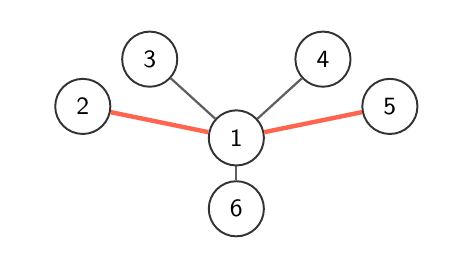
\begin{tikzpicture}[x=1cm,y=1cm]
        \node[graphvertex] (s1) at (2.25,0) {1};
        \foreach \i/\x/\y in {2/0.3/0.4,3/1.15/1.0,4/3.35/1.0,5/4.2/0.4,6/2.25/-0.9}
          {\node[graphvertex] (s\i) at (\x,\y) {\i};}
        \foreach \i in {3,4,6} {\draw[graphedge] (s1)--(s\i);}
        \foreach \i in {2,5}
          {\draw[draw=vnaccent,line width=1.6pt] (s1)--(s\i);}
        \path[use as bounding box] (-0.4,-1.3) rectangle (4.9,1.4);
      \end{tikzpicture}
\end{document}
